\documentclass{beamer}
\usetheme{metropolis}
\usepackage{graphicx}
\usepackage[normalem]{ulem}
\usepackage[french]{babel}
\usepackage{marvosym}
\usepackage{qrcode}
% Horizontal lists
% \usepackage[inline]{enumitem}
\usepackage{minted}

% -- ChatGPTeries pour slide dorée --%
\usepackage{tikz}
\usepackage{xcolor}

\definecolor{gold}{RGB}{201, 164, 76}
\definecolor{darkgold}{RGB}{142, 111, 35}
\definecolor{luxuryblack}{RGB}{18, 18, 18}
\definecolor{softwhite}{RGB}{242, 240, 234}
% ---- %

\usepackage{tikz}
\usepackage{xcolor}
\usetikzlibrary{positioning, calc, shapes.geometric}

% -- Icones pour la slide "langage de haut niveau" -- %
% Baguette magique : image demandee par l'utilisateur (istockphoto, a
% verifier niveau licence avant toute diffusion publique des slides).
\newcommand{\wandicon}{.}
\newcommand{\screenicon}{%
	\begin{tikzpicture}[baseline=-0.3ex, scale=0.35]
		\draw[thick, fill=black!5] (-1,0) rectangle (1,0.7);
		\node[font=\tiny] at (0,0.35) {Salut};
		\draw[thick] (-0.15,-0.35) rectangle (0.15,0);
		\draw[thick] (-0.5,-0.5) -- (0.5,-0.5);
	\end{tikzpicture}%
}
% ---- %

% Slides année précédente
\usetikzlibrary{positioning, calc, decorations.pathreplacing}

\definecolor{pillfill}{RGB}{173, 216, 240}
\definecolor{pillborder}{RGB}{70, 130, 180}
\tikzset{
  pill/.style={draw=pillborder, thick, rounded corners=8pt, fill=pillfill,
    minimum height=0.8cm, text width=3.6cm, align=center, font=\bfseries\small},
  pillsmall/.style={draw=pillborder, thick, rounded corners=6pt, fill=pillfill,
    minimum height=0.7cm, text width=2.6cm, align=center, font=\bfseries\footnotesize},
}

% -- Coloration syntaxique du code Python (compatible pdflatex) -- %
\usepackage{listings}
% Quickfix to get Listings to work properly
% From https://tex.stackexchange.com/questions/451532/recent-issues-with-lstlinebgrd-package-with-listings-after-the-latters-updates
\makeatletter
\let\old@lstKV@SwitchCases\lstKV@SwitchCases
\def\lstKV@SwitchCases#1#2#3{}
\makeatother
\usepackage{lstlinebgrd}
\makeatletter
\let\lstKV@SwitchCases\old@lstKV@SwitchCases

\lst@Key{numbers}{none}{%
    \def\lst@PlaceNumber{\lst@linebgrd}%
    \lstKV@SwitchCases{#1}%
    {none:\\%
     left:\def\lst@PlaceNumber{\llap{\normalfont
                \lst@numberstyle{\thelstnumber}\kern\lst@numbersep}\lst@linebgrd}\\%
     right:\def\lst@PlaceNumber{\rlap{\normalfont
                \kern\linewidth \kern\lst@numbersep
                \lst@numberstyle{\thelstnumber}}\lst@linebgrd}%
    }{\PackageError{Listings}{Numbers #1 unknown}\@ehc}}
\makeatother
\definecolor{codekw}{RGB}{0, 0, 180}
\definecolor{codestr}{RGB}{20, 120, 40}
\definecolor{codecom}{RGB}{120, 120, 120}
\lstdefinestyle{python}{
	language=Python,
	basicstyle=\ttfamily\footnotesize,
	keywordstyle=\color{codekw}\bfseries,
	stringstyle=\color{codestr},
	commentstyle=\color{codecom}\itshape,
	showstringspaces=false,
	keepspaces=true,
	columns=fullflexible,
	aboveskip=0pt,
	belowskip=0pt,
	literate={é}{{\'e}}1 {è}{{\`e}}1 {ê}{{\^e}}1 {à}{{\`a}}1 {ç}{{\c c}}1
	{É}{{\'E}}1 {'}{{\textquotesingle}}1,
}
\lstdefinestyle{pythonsmall}{style=python,basicstyle=\ttfamily\scriptsize}

% Convention du cours pour une reponse de Python (a la suite d'un print, etc.) :
% prefixe ">" + encadre sur fond clair.
\lstdefinestyle{pythonoutput}{
	style=python,
	basicstyle=\ttfamily\footnotesize\color{black!70},
	backgroundcolor=\color{black!6},
	frame=single,
	rulecolor=\color{black!35},
	framerule=0.4pt,
	framexleftmargin=5pt,
	framexrightmargin=5pt,
	framextopmargin=3pt,
	framexbottommargin=3pt,
	xleftmargin=5pt,
	xrightmargin=5pt,
	aboveskip=3pt,
	belowskip=3pt,
}

% Un morceau de code annote : #1 plage de lignes, #2 1 si c'est la partie
% commentee (fond bleu, couleurs normales) sinon 0 (grise), #3 aboveskip.
\newcommand{\annoline}[3]{%
	\ifnum#2=1
	\lstinputlisting[style=pythonsmall, backgroundcolor=\color{blue!15}, #3, linerange={#1}]{code/premier_prog_2.py}%
	\else
	\lstinputlisting[style=pythonsmall, basicstyle=\ttfamily\scriptsize\color{black!45}, keywordstyle=\color{black!45}, stringstyle=\color{black!45}, #3, linerange={#1}]{code/premier_prog_2.py}%
	\fi
}

% Version generique de \annoline : #1 fichier, #2 plage de lignes,
% #3 1 si c'est la ligne commentee (fond bleu) sinon 0 (grisee).
\newcommand{\valline}[3]{%
	\ifnum#3=1
	\lstinputlisting[style=pythonsmall, backgroundcolor=\color{blue!15}, linerange={#2}]{#1}%
	\else
	\lstinputlisting[style=pythonsmall, basicstyle=\ttfamily\scriptsize\color{black!45}, keywordstyle=\color{black!45}, stringstyle=\color{black!45}, linerange={#2}]{#1}%
	\fi
}

% Slide "focus sur une construction" : etape 1 = programme entier, la partie
% commentee sur fond bleu (texte noir), le reste gris ; etape 2 = le reste a
% disparu, la partie commentee reste sur fond bleu (texte noir).
\newcommand{\focusframe}[5]{%
	\begin{frame}[t]{#1}
		\only<1>{\lstinputlisting[
			style=pythonsmall,
			basicstyle=\ttfamily\scriptsize\color{black!45},
			keywordstyle=\color{black!45}, stringstyle=\color{black!45},
			emph={#2}, emphstyle={\color{black}\bfseries},
			linebackgroundcolor={\color{white}#3},
			]{code/premier_prog_2.py}}%
		\only<2>{\lstinputlisting[
			style=pythonsmall,
			emph={#2}, emphstyle={\color{black}\bfseries},
			linebackgroundcolor={\color{white}#3},
			]{code/#4}}%
		\vfill
		\centering\small #5
	\end{frame}%
}

\title{Algorithmique et Programmation 1}
\author{A. Boussidan, L. Exibard, P. Yvonnet}
\date{21 Septembre 2026}

\begin{document}

\begin{frame}
    \maketitle
\end{frame}

\begin{frame}{Quelques questions pour commencer !}

  cf \href{https://app.wooclap.com/events/PUTHMFD}{Wooclap}.

\end{frame}

\section{Dans les épisodes précédents...}

\begin{frame}[t]{Qu'est-ce qu'une variable ?}
  \pause
	\begin{center}
		Une valeur est une boîte dans laquelle on range quelque chose.
	\end{center}

	\begin{center}\texttt{x = 2}\end{center}%

	\begin{center}
		\begin{tikzpicture}
			\node (boite) {
\includegraphics[width=3.6cm]{Images/Carton fermé_x.png}};%
		\end{tikzpicture}
	\end{center}
\end{frame}

\begin{frame}{Mais encore ?}

  \begin{block}{Variable}
    \vspace{0pt}
    Une variable est :
    \begin{itemize}
      \item un \emph{nom}
      \item associé à une \emph{valeur} en mémoire
      \item via l'opération d'affectation \texttt{=}
      \end{itemize}
    \end{block}
  \MVRightarrow{} Une variable stocke des \emph{données}
\end{frame}

\begin{frame}[t]{Que peut-on mettre dans une variable ?}
  \pause
		\begin{center}
			\begin{tikzpicture}[font=\small]
        \onslide<1-2>{
				\node at (-4.5,2.2) {Une note};
				\node at (-1.2,2.4) {Une moyenne};
				\node at (-4.5,1.0) {Un nombre de notes};
				\node at (2.8,2.4) {\color{codestr}"Salut"};
				\node at (-4.5,-0.2) {2};
				\node at (0.8,-3.3) {Plein de notes différentes};
				\node at (-1.2,-1.6) {Si on a fini de saisir};
				\node at (2.8,1.0) {\color{codestr}"Entrez une note"};
				\node at (2.8,-1.6) {Rien du tout};
        }

        \onslide<1-2>{\draw[thick, red, rounded corners=8pt] (-6.1,-0.7) rectangle (-3.0,2.7);}
					\onslide<1-3>{\node[font=\bfseries] at (-4.55,-1.15) {Entiers : \texttt{int}};}
				% etape 13 : flottants (label sur 2 lignes pour ne pas deborder sur les chaines)
					\onslide<1-2>{\draw[thick, red, rounded corners=8pt] (-2.3,2.0) rectangle (-0.1,2.9);}
          \onslide<1-3>{\node[font=\bfseries, anchor=north west, align=left] at (-2.9,1.85) {Nombres à virgule :\\\texttt{float}};}
				% etape 14 : booleens
					\onslide<1-2>{\draw[thick, red, rounded corners=8pt] (-2.7,-2.0) rectangle (0.3,-1.2);}
					\onslide<1-3>{\node[font=\bfseries] at (-1.2,-2.4) {Vrai/Faux : \texttt{bool}};}
				% etape 15 : chaines de caracteres
					\onslide<1-2>{\draw[thick, red, rounded corners=8pt] (1.5,0.5) rectangle (4.4,2.9);}
					\onslide<1-3>{\node[font=\bfseries] at (2.95,0.1) {Texte : \texttt{str}};}
				% etape 16-17 : NoneType (?? puis NoneType) - rectangle agrandi pour contenir tout le texte
					\onslide<1-2>{\draw[thick, red, rounded corners=8pt] (1.3,-2.0) rectangle (4.3,-1.2);}
					\onslide<1-3>{\node[font=\bfseries] at (2.8,-2.4) {\texttt{NoneType}};}
				% etape 18 : listes
					\onslide<1-2>{\draw[thick, red, rounded corners=8pt] (-2.2,-3.7) rectangle (3.8,-2.9);}
					\onslide<1-3>{\node[font=\bfseries] at (0.8,-4.1) {Liste : \texttt{list}};}
			\end{tikzpicture}
		\end{center}
\end{frame}

\begin{frame}{Que peut-on mettre dans une variable ? Les types}
  \begin{block}{Types}
    \vspace{0pt}
    En Python, les types \emph{primitifs} sont :
    \vspace{-0.5em}
    \begin{description}
    \item[Entiers] \texttt{int}
    \item[Nombres à virgule] \texttt{float}
    \item[Texte] \texttt{str}
    \item[Vrai/faux] \texttt{bool}
    \item[Rien] \texttt{NoneType}
    \end{description}
    \pause
    Les types \emph{construits} (ou \emph{containers}) sont :
    \vspace{-0.5em}
    \begin{description}
    \item[Liste de valeurs] \texttt{list}
      \pause
    \item[Tuples de valeurs] \texttt{tuple} (on verra plus tard)
    \item[Dictionnaires] \texttt{dict} (on verra plus tard)
    \end{description}
    \MVRightarrow{} Ils servent à \emph{grouper} des valeurs
  \end{block}
\end{frame}

\begin{frame}[t]{Manipuler les valeurs}
	\begin{columns}[T]
		\begin{column}{0.55\textwidth}
			\only<1>{\valline{code/echange_valeurs.py}{1-1}{1}\valline{code/echange_valeurs.py}{2-5}{0}}%
			\only<2->{\valline{code/echange_valeurs.py}{1-4}{0}\valline{code/echange_valeurs.py}{5-5}{1}}%
		\end{column}
		\begin{column}{0.4\textwidth}
			\begin{center}
				\renewcommand{\arraystretch}{1.3}
				\begin{tabular}{cc}
					\texttt{a} & \texttt{b} \\ \hline
					\onslide<1->{\texttt{3} & \texttt{---} \\}
          \onslide<2->{%
					\texttt{3} & \texttt{5} \\
					\texttt{8} & \texttt{5} \\
					\texttt{8} & \texttt{3} \\
					\texttt{5} & \texttt{3} \\}
				\end{tabular}
			\end{center}
		\end{column}
	\end{columns}
		\begin{center}
      \onslide<2->{%
			\textbf{Ce code échange les deux valeurs, sans variable auxiliaire !}
      }
		\end{center}
\end{frame}

\section{Les expressions}

\begin{frame}[t]{Manipuler les valeurs}
	\begin{columns}[T]
		\begin{column}{0.55\textwidth}
			\valline{code/echange_valeurs.py}{1-4}{0}\valline{code/echange_valeurs.py}{5-5}{1}
		\end{column}
		\begin{column}{0.4\textwidth}
		\end{column}
	\end{columns}
\end{frame}

\begin{frame}{Manipuler les valeurs : les expressions}
  \begin{block}{Expression}
    \vspace{0pt}
  Une expression :

  \begin{itemize}
    \item est une combinaison de valeurs, variables et opérateurs
    \item peut s'évaluer
    \item a donc une valeur
    \item (et donc un type !)
    \end{itemize}
    \end{block}

    \begin{exampleblock}{Exemples}
      \vspace{0pt}
        \mintinline{python}{"Coucou"}
          \pause
        \qquad \mintinline{python}{3}
          \pause
        \qquad \mintinline{python}{False}
          \pause
        \qquad \mintinline{python}{1 + 2 * 3}
          \pause
        \qquad \mintinline{python}{"cou" * 2}
          \pause
        \qquad \mintinline{python}{True and True or False}
          \pause
        \qquad \mintinline{python}{z + 5 > 128}
          \pause
        \qquad \mintinline{python}{"cou" * 2 == "cou" + "cou"}
          \pause
        \qquad \mintinline{python}{x == 8}
          \pause
        \qquad \alt<1-10>{\mintinline{python}{x = 8}}{\sout{\mintinline{python}{x = 8}}}
        \pause
      \end{exampleblock}
\end{frame}



\begin{frame}[t]{Qu'est-ce qu'il y a dans ce programme ?}
	\lstinputlisting[style=pythonsmall]{code/premier_prog_2.py}%
\end{frame}

\focusframe{Conditions : si\dots{} sinon}{if,else}{%
	\ifnum\value{lstnumber}>5\ifnum\value{lstnumber}<11 \color{codekw!12}\fi\fi
}{focus_ifelse.py}{\textbf{Choisir} selon une condition.}

\section{Les booléens}

\begin{frame}{Les booléens : \texttt{bool}}
  \begin{columns}
    \begin{column}{0.7\textwidth}
        \mintinline{python}{False}
        \qquad \mintinline{python}{True and True or False}
        \qquad \mintinline{python}{z + 5 > 128}
        \qquad \mintinline{python}{"cou" * 2 == "cou" + "cou"}
        \qquad \mintinline{python}{x == 8}
        \pause

        \bigskip

        \mintinline{python}{nouvelle_note < 0 or nouvelle_note > 20}
    \end{column}
    \begin{column}{0.3\textwidth}
      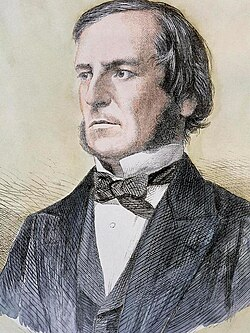
\includegraphics[width=\textwidth]{Images/George_Boole_color.jpg}

      \begin{center}
      George Boole
      \end{center}
    \end{column}
    \end{columns}
\end{frame}

\begin{frame}{Les booléens : \texttt{bool}}

  \begin{block}{Booléen}
    \vspace{0pt}
    Les booléens sont :

    \begin{itemize}
    \item un type de données
    \item qui a seulement deux éléments :
      \begin{itemize}
        \item \mintinline{python}{True}
        \item \mintinline{python}{False}
      \end{itemize}
    \item et permet d'évaluer la \emph{valeur de vérité d'expressions}
    \end{itemize}
    \MVRightarrow{} Exprime une \alert{condition}.
  \end{block}
\end{frame}

\begin{frame}{Les booléens : \texttt{bool}}

  \begin{block}{Valeurs booléennes}
    \vspace{0pt}
      \begin{itemize}
        \item \mintinline{python}{True} (1, vrai)
        \item \mintinline{python}{False} (0, faux)
      \end{itemize}
  \end{block}

  \begin{block}{Opérateurs booléens}
    \vspace{0pt}
      \begin{itemize}
        \item \mintinline{python}{not} (non)
        \item \mintinline{python}{and} (et)
        \item \mintinline{python}{or} (ou)
      \end{itemize}
  \end{block}

  \begin{exampleblock}{Exemples}
    \vspace{0pt}
    \mintinline{python}{not False}
    \qquad \mintinline{python}{False and True}
    \qquad \mintinline{python}{False or True}
    \qquad \mintinline{python}{not (False and True)}
    \qquad \mintinline{python}{not ((True or False) and (False and False))}
  \end{exampleblock}
\end{frame}

\begin{frame}{Les booléens : \texttt{bool}}
  \begin{block}{Expressions booléennes}
    \vspace{0pt}
    Les expressions booléennes :
    \begin{itemize}
    \item s'évaluent à \mintinline{python}{True} ou \mintinline{python}{False}
    \item sont construites avec :
      \begin{itemize}
      \item les opérateurs booléens
        \pause
      \item les opérateurs de comparaison :

    \qquad \mintinline{python}{==}
    \qquad \mintinline{python}{!=}
    \qquad \mintinline{python}{<}
    \qquad \mintinline{python}{>}
    \qquad \mintinline{python}{<=}
    \qquad \mintinline{python}{>=}
      \end{itemize}
    \end{itemize}

  \begin{exampleblock}{Exemples}
    \vspace{0pt}
        \mintinline{python}{z + 5 > 128}
        \qquad \mintinline{python}{"cou" * 2 == "cou" + "cou"}
        \qquad \mintinline{python}{x != 8}
        \qquad \mintinline{python}{nouvelle_note < 0 or nouvelle_note > 20}
  \end{exampleblock}
  \end{block}
\end{frame}

\section{Conditionnelles \mintinline{python}{if} ... \mintinline{python}{else}}

\begin{frame}{Dessiner des polygones : le retour}

\pause

\bigskip

	\lstinputlisting[style=pythonsmall]{code/polygones_full_compact.py}%
\end{frame}

\begin{frame}{Structures de contrôle}

  Jusqu'à présent, on n'a fait que des \emph{séquences d'instructions}.

  \begin{block}{Branchement conditionnel}
    \vspace{0pt}
    Les structures conditionnelles :
    \begin{itemize}
    \item gèrent l'ordre d'exécution des instructions
    \item évaluent des \emph{expressions booléennes}
    \item permettent de \emph{brancher} dans le code.
    \end{itemize}
  \end{block}
\end{frame}
\begin{frame}{Branchement conditionnel \mintinline{python}{if} ... \mintinline{python}{else} (ou \emph{si} ... \emph{alors} ... \emph{sinon})}
  \begin{columns}
    \begin{column}{0.7\textwidth}
  \scalebox{0.8}{%
\begin{tikzpicture}[
    every node/.style={font=\small},
    process/.style={
        rectangle,
        draw,
        rounded corners,
        minimum width=3cm,
        minimum height=1cm,
        align=center
    },
    decision/.style={
        diamond,
        draw,
        aspect=2,
        minimum width=2.8cm,
        align=center
    },
    arrow/.style={
        ->,
        >=stealth
    }
]

% Blocs
\node[process] (debut) {Début};
\node[decision, below=of debut] (condition) {Condition ?};

\node[process, below left=2cm and 0.5cm of condition] (oui) {Action si vrai};
\node[process, below right=2cm and 0.5cm of condition] (non) {Action si faux};

\node[process, below=4.5cm of condition] (suite) {Suite du programme};

% Flèches
\draw[arrow] (debut) -- (condition);

\draw[arrow] (condition) -- node[above left] {oui} (oui);
\draw[arrow] (condition) -- node[above right] {non} (non);

\draw[arrow] (oui) -- (suite);
\draw[arrow] (non) -- (suite);

\end{tikzpicture}
}
\end{column}
\begin{column}{0.3\textwidth}
	\lstinputlisting[style=pythonsmall]{code/if_else.py}%
  \end{column}
  \end{columns}

\end{frame}

\section{Intermède : bonnes pratiques de codage}

\begin{frame}{L'indentation}

  \pause

  En Python, l'espacement par rapport à la marge a une importance !

  \MVRightArrow{} On appelle ça \emph{l'indentation}.

  \begin{exampleblock}{Exemple}
	\lstinputlisting[style=pythonsmall]{code/indentation.py}%
  \end{exampleblock}

\end{frame}



% ------------------------------------------------------------------
% Slide "Les règles d'or"
% ------------------------------------------------------------------

\begin{frame}[plain]

\begin{tikzpicture}[remember picture, overlay]

  % Fond
  \fill[luxuryblack] (current page.south west)
      rectangle (current page.north east);

  % Double filet doré, rapproché des bords
  \draw[gold, line width=0.8pt]
      ([xshift=0.28cm,yshift=0.28cm]current page.south west)
      rectangle
      ([xshift=-0.28cm,yshift=-0.28cm]current page.north east);

  \draw[darkgold, line width=0.3pt]
      ([xshift=0.43cm,yshift=0.43cm]current page.south west)
      rectangle
      ([xshift=-0.43cm,yshift=-0.43cm]current page.north east);

  % Petit ornement central
  \node[gold, font=\large] at
      ([yshift=-0.95cm]current page.north)
      {$\diamond$};

  % Titre
  \node[
      anchor=north,
      text=gold,
      font=\fontsize{21}{25}\selectfont\bfseries
  ] at ([yshift=-1.25cm]current page.north)
  {LES RÈGLES D'OR d'AP1};

  % Ligne décorative
  \draw[gold, line width=0.5pt]
      ([xshift=-2.3cm,yshift=-2.15cm]current page.north)
      -- ([xshift=2.3cm,yshift=-2.15cm]current page.north);
  % ================================================================
  % RÈGLE 01
  % ================================================================

  \node[
      anchor=north west,
      text=gold,
      font=\fontsize{12}{14}\selectfont\bfseries
  ] at ([xshift=1.15cm,yshift=-2.85cm]current page.north west)
  {01};

  \node[
      anchor=north west,
      text=softwhite,
      font=\normalsize\bfseries
  ] at ([xshift=2.05cm,yshift=-2.80cm]current page.north west)
  {Être un chef.};

  \node[
      anchor=north west,
      text=softwhite!70,
      font=\footnotesize
  ] at ([xshift=2.05cm,yshift=-3.30cm]current page.north west)
  {Penser à l'algorithme avant de programmer};

  % ================================================================
  % RÈGLE 02
  % ================================================================

  \node[
      anchor=north west,
      text=gold,
      font=\fontsize{12}{14}\selectfont\bfseries
  ] at ([xshift=1.15cm,yshift=-4cm]current page.north west)
  {02};

  \node[
      anchor=north west,
      text=softwhite,
      font=\normalsize\bfseries
  ] at ([xshift=2.05cm,yshift=-4.05cm]current page.north west)
  {Connaître ses ingrédients.};

  \node[
      anchor=north west,
      text=softwhite!70,
      font=\footnotesize
  ] at ([xshift=2.05cm,yshift=-4.55cm]current page.north west)
  {Penser au type de chaque variable};

  % ================================================================
  % RÈGLE 03
  % ================================================================

\pause
  \node[
      anchor=north west,
      text=gold,
      font=\fontsize{12}{14}\selectfont\bfseries
  ] at ([xshift=1.15cm,yshift=-5.2cm]current page.north west)
  {03};

  \node[
      anchor=north west,
      text=softwhite,
      font=\normalsize\bfseries
  ] at ([xshift=2.05cm,yshift=-5.25cm]current page.north west)
  {Soigner le dressage.};

  \node[
      anchor=north west,
      text=softwhite!70,
      font=\footnotesize
  ] at ([xshift=2.05cm,yshift=-5.75cm]current page.north west)
  {Penser à l'indentation};

  % ================================================================
  % Pied de page
  % ================================================================

  \node[
      anchor=south,
      text=gold!80,
      font=\tiny\scshape
  ] at ([yshift=0.75cm]current page.south)
  {À retenir};

\end{tikzpicture}

\end{frame}

\begin{frame}{Les différents modes de Python}

  \pause

  \begin{block}{Le mode interactif : REPL}
    \vspace{0pt}
    REPL = \emph{Read Evaluate Print Loop}

    \MVRightarrow{} Python exécute les commandes et affiche le résultat \emph{au fur et à mesure}
    \end{block}

  \begin{block}{Le mode exécutable : console}
    \vspace{0pt}
    On exécute un programme Python

    \MVRightarrow{} Python exécute le programme \emph{d'un seul coup}
    \end{block}

\end{frame}


\section{La boucle \mintinline{python}{while}}

\begin{frame}{Branchement conditionnel \emph{répété} \mintinline{python}{while} (ou \emph{tant que} ... \emph{faire})}

  Que faire si on veut répéter une instruction si une condition reste vraie ?

  \begin{columns}
    \begin{column}{0.7\textwidth}
  \scalebox{0.8}{%
\begin{tikzpicture}[
    every node/.style={font=\small},
    process/.style={
        rectangle,
        draw,
        rounded corners,
        minimum width=3cm,
        minimum height=1cm,
        align=center
    },
    decision/.style={
        diamond,
        draw,
        aspect=2,
        minimum width=3cm,
        minimum height=1.2cm,
        align=center
    },
    arrow/.style={
        ->,
        >=stealth,
        thick
    }
]

% Blocs
\node[process] (debut) {Début};

\node[decision, below=1.2cm of debut] (condition) {Condition ?};

\node[process, below=1.5cm of condition] (bloc) {Bloc};

\node[process, below=1.5cm of bloc] (suite) {Suite du programme};


% Début -> Condition
\draw[arrow]
    (debut) -- (condition);


% Condition -> Bloc : OUI
\draw[arrow]
    (condition.south)
    -- node[right] {oui}
    (bloc.north);


% Bloc -> Condition : retour de la boucle
\draw[arrow]
    (bloc.west)
    -- ++(-2cm,0)
    |- node[left, pos=0.25] {}
    (condition.west);


% Condition -> Suite : NON
\draw[arrow]
    (condition.east)
    to[out=0, in=0]
    node[right] {non}
    (suite.east);

\end{tikzpicture}

% \begin{tikzpicture}[
%     every node/.style={font=\small},
%     process/.style={
%         rectangle,
%         draw,
%         rounded corners,
%         minimum width=3cm,
%         minimum height=1cm,
%         align=center
%     },
%     decision/.style={
%         diamond,
%         draw,
%         aspect=2,
%         minimum width=2.8cm,
%         align=center
%     },
%     arrow/.style={
%         ->,
%         >=stealth
%     }
% ]

% % Blocs
% \node[process] (debut) {Début};
% \node[decision, below=of debut] (condition) {Condition ?};
% \node[process, below=of condition] (bloc) {Bloc};
% \node[process, below=of bloc] (suite) {Suite du programme};

% % Flèches
% \draw[arrow] (debut) -- (condition);

% \draw[arrow, bend right] (condition) -- node[above left] {oui} (bloc);
% \draw[arrow, bend left] (condition) -- node[above right] {non} (suite);

% \end{tikzpicture}
}
\end{column}
\begin{column}{0.3\textwidth}
	\lstinputlisting[style=pythonsmall]{code/while.py}%
  \end{column}
  \end{columns}
\end{frame}

\begin{frame}{Dessiner des polygones : le \emph{re}-retour}

\pause

\bigskip

	\lstinputlisting[style=pythonsmall]{code/polygones_full_compact.py}%
\end{frame}

\section{Les listes}

\end{document}

%%% Local Variables:
%%% TeX-engine: xetex
%%% TeX-command-extra-options: "-shell-escape"
%%% End:
